%%%%%%%%%%%%%%%%%%%%%%%%%%%%%%%%%%%%%%%%%
% Dreuw & Deselaer's Poster
% LaTeX Template
% Version 1.0 (11/04/13)
%
% Created by:
% Philippe Dreuw and Thomas Deselaers
% http://www-i6.informatik.rwth-aachen.de/~dreuw/latexbeamerposter.php
%
% This template has been downloaded from:
% http://www.LaTeXTemplates.com
%
% License:
% CC BY-NC-SA 3.0 (http://creativecommons.org/licenses/by-nc-sa/3.0/)
%
%%%%%%%%%%%%%%%%%%%%%%%%%%%%%%%%%%%%%%%%%

%----------------------------------------------------------------------------------------
%	PACKAGES AND OTHER DOCUMENT CONFIGURATIONS
%----------------------------------------------------------------------------------------

\documentclass[final,hyperref={pdfpagelabels=false}]{beamer}

\usepackage[orientation=portrait,size=a0,scale=1.4]{beamerposter} % Use the beamerposter package for laying out the poster with a portrait orientation and an a0 paper size

\usetheme{I6pd2} % Use the I6pd2 theme supplied with this template

\usepackage[english]{babel} % English language/hyphenation

\usepackage{amsmath,amsthm,amssymb,latexsym} % For including math equations, theorems, symbols, etc

%\usepackage{times}\usefonttheme{professionalfonts}  % Uncomment to use Times as the main font
%\usefonttheme[onlymath]{serif} % Uncomment to use a Serif font within math environments

\boldmath % Use bold for everything within the math environment

\usepackage{booktabs} % Top and bottom rules for tables

\graphicspath{{figures/}} % Location of the graphics files

\usecaptiontemplate{\small\structure{\insertcaptionname~\insertcaptionnumber: }\insertcaption} % A fix for figure numbering

%----------------------------------------------------------------------------------------
%	TITLE SECTION 
%----------------------------------------------------------------------------------------

\title{\huge The Ion Trap Architecture} % Poster title

\author{Atul Singh Arora} % Author(s)

\institute{Indian Institute of Science, Education and Research, Mohali} % Institution(s)

%----------------------------------------------------------------------------------------
%	FOOTER TEXT
%----------------------------------------------------------------------------------------

\newcommand{\leftfoot}{http://www.github.com/toAtularora} % Left footer text

\newcommand{\rightfoot}{to.AtulArora@gmail.com} % Right footer text

%----------------------------------------------------------------------------------------

\begin{document}

\addtobeamertemplate{block end}{}{\vspace*{2ex}} % White space under blocks

\begin{frame}[t] % The whole poster is enclosed in one beamer frame

\begin{columns}[t] % The whole poster consists of two major columns, each of which can be subdivided further with another \begin{columns} block - the [t] argument aligns each column's content to the top

\begin{column}{.02\textwidth}\end{column} % Empty spacer column

\begin{column}{.465\textwidth} % The first column

%----------------------------------------------------------------------------------------
%	Prerequisites
%----------------------------------------------------------------------------------------

\begin{block}{Prerequisites}

	% Can read and take being made fun of occasionally in good spirit. Also
	% it'll help if you have some rough idea about what qubits etc. really
	% are and their use in the context of information processing. qubits
	Basic knowledge of physical concepts. A rough idea about qubits will be helpful; infact knowing that they reside in the space spanned by the states of any two level quantum system is sufficient.

\end{block}

%----------------------------------------------------------------------------------------
%	INTRODUCTION
%----------------------------------------------------------------------------------------
            
\begin{block}{Confining the ions}
	If you've read Griffiths with any love, you would know that Earnshaw's
	theorem prohibits creation of a minima using electrostatic potential.
	(now don't ask which Griffiths) Thus you can't trap ions conventionally.
	% \begin{enumerate}
	% \item Confining the ions

	\begin{enumerate}
		\item Production of ions: It involves heating calcium in high vacuum, then firing of high speed electrons on its vapour. Consequently some resulting ions fall inside the trap and get stuck.

		\begin{figure}
		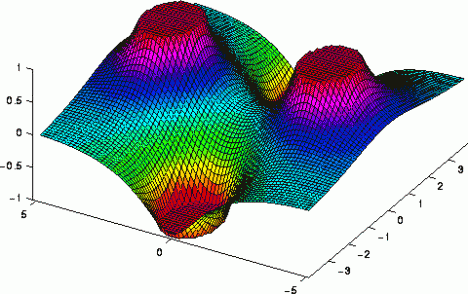
\includegraphics[width=0.8\linewidth]{potential}
		\caption{Potential in space [1]}
		\end{figure}

		\item Trap structure: The idea is simple. Since you can't create a potential minima anywhere
		inside the boundary, you can't trap an ion. But you see the saddle
		point. (In the figure, the X and Y axis represent physical space and Z is the potential.) You change the potential rapidly so that the `U' minima oscillates
		between being along the X and Y axis (say). (The flat circular part is the electrode's surface) This way, on an average,
		the saddle point sees zero average potential. If the ion was anywhere
		other than this point, it'll experiences oscillating forces. This
		effectively results in confinement of the atom. Q1. How does an oscillating
		force ensure confinement? Q2. What frequencies are most effective
		and why? Q3. How do you know only 1 ion is trapped? \\
		The next immediate question is what restricts the ion in the spatial Z axis.
		Well, we just pin the ion using a positive potential (by putting two
		electrodes along the said axis.)

	\end{enumerate}

\end{block}

%----------------------------------------------------------------------------------------
%	Control
%----------------------------------------------------------------------------------------
\begin{block}{Ion Control}
	\begin{enumerate}
		\item Let's say that it is obvious we need the kinetic energy of the ions
		to be much smaller than that it picks up upon interaction with a laser
		(or upon emitting a single photon). This number turns up to be about
		32 K Hertz (Energy/Plank's constant). The corresponding temperature
		to have thermal energy lower than this, turns out to be a few micro
		kelvins!\\
		This is a serious challenge.
		\item How do you circumvent this? Laser cooling. Oxymoron you might say
		but the following little thought is illuminating. If you hit an atom
		with light with opposite momentum, the atom slows down as the light
		is bounced back. So if you could get the ions to absorb light preferentially
		going opposite in direction to their momentum, you've found a ground-breaking
		method of cooling!\\
		And yes, somebody thought of that too. You use something you're already
		familiar with, resonance and Doppler.

		\begin{enumerate}
			\item Resonance: This is the (in)famous phenomenon where an innocent and
			mild vibration can cause an otherwise stable system to have almost
			devastating effects, given the frequency is just right. A similar
			effect is observed with atoms and with remarkable sensitivity to the
			precision of the frequency. Light is absorbed by the atom only when
			the frequency is just right.
			\item Doppler: This is as you're well aware, the principle behind the sound
			effect you get when a car zooms past. We exploit this and set the
			frequency of the laser just below the resonant frequency. This does
			it then.\\		
		\end{enumerate}
		NOTE: This is not at all this simple. Q1. If the photon is absorbed,
		it must be emitted giving the atom a push again! What's wrong? Q2.
		What about line broadening etc.?		
	\end{enumerate}

\end{block}

% \begin{block}{Ion Control}

% \begin{columns} % Subdivide the first main column
% \begin{column}{.54\textwidth} % The first subdivided column within the first main column
% \begin{itemize}
% \item Vestibulum nisl, quis euismod velit eros in ligula.
% \begin{itemize}
% \item Cras rhoncus quam et augue convallis in elementum urna tincidunt.
% \end{itemize}
% \item Proin ut vestibulum augue.
% \begin{itemize}
% \item Donec dapibus sagittis neque eu ultrices.
% \end{itemize}
% \end{itemize}
% \end{column}

% \begin{column}{.43\textwidth} % The second subdivided column within the first main column
% \centering
% \begin{figure}
% 
\includegraphics[width=0.8\linewidth]{placeholder.jpg}
% \caption{Figure caption}
% \end{figure}
% \end{column}
% \end{columns} % End of the subdivision

% \begin{itemize}
% \item Curabitur sapien ligula, faucibus in feugiat quis, vestibulum a turpis.
% \begin{itemize}
% \item Phasellus quis nunc neque. Suspendisse mauris diam, suscipit non gravida in, placerat id enim. Ut nec ipsum in lectus ultrices sagittis.
% \item Ut nec ipsum in lectus ultrices sagittis.
% \item Phasellus quis nunc neque.
% \end{itemize}
% \end{itemize}

% \end{block}

%----------------------------------------------------------------------------------------
%	METHODS
%----------------------------------------------------------------------------------------

% \begin{block}{Methods}

% \begin{itemize}
% \item Maecenas Vel Nisl Elit
% \begin{itemize}
% \item Suspendisse potenti. Fusce a est eget turpis rhoncus varius sed sed dui. Cras justo nibh, bibendum a cursus eget, consequat et dui. Maecenas vel nisl elit, sed dignissim dolor. 
% \item In hac habitasse platea dictumst.
% \end{itemize}

% \item Viewpoint Matching Constraints
% \begin{itemize}
% \item Cum sociis natoque penatibus et magnis dis parturient montes, nascetur ridiculus mus. 
% \item Proin in nisi diam.
% \item Nam ultricies pellentesque nunc, ultrices volutpat nisl ultrices a.
% \end{itemize}

% \item Volutpat 
% \begin{itemize}
% \item Duis semper lorem eget dui dignissim porttitor.
% \item Nulla facilisi. In ullamcorper lorem quis dolor.
% \end{itemize}
% \end{itemize}

% \end{block}

% %----------------------------------------------------------------------------------------
% %	MATHEMATICAL SECTION
% %----------------------------------------------------------------------------------------

% \begin{block}{Mathematical Section}

% \begin{itemize}
% \item Maecenas Ultricies Feugiat Velit Non Mattis.
% \begin{itemize}
% \item Duis ante erat, bibendum nec tempus nec, interdum quis est. Nulla at mollis tortor. Phasellus quis leo dolor, aliquam laoreet orci $X$ Donec dapibus sagittis neque eu nec, interdum quis est. $Y_n, n=1,\cdots,N$ ndum nec tempus nec, interd
% \begin{align*}
% X \rightarrow r(X) & = \arg \max_{c} \Big\{ \max_n \big\{ \sum_{x_i \in X} \delta(x_i,Y_{n,c})\big\} \Big\} 
% \end{align*}
% \item Cras faucibus scelerisque cursus. Proin ut vestibulum augue. $\delta(x_i,Y_{n,c})$
% \end{itemize}
% \item Fusce tempus arcu id ligula varius dictum. Donec ut nisl dui, ac consectetur elit. In nec enim porta augue venenatis sollicitudin. Phasellus quis nunc neque. Suspendisse mauris diam, suscipit non gravida in, placerat id enim. Ut nec ipsum in lectus ultrices sagittis.
% \end{itemize}

% \end{block}

% %----------------------------------------------------------------------------------------

\end{column} % End of the first column

\begin{column}{.03\textwidth}\end{column} % Empty spacer column
 
\begin{column}{.465\textwidth} % The second column

%----------------------------------------------------------------------------------------
%	RESULTS
%----------------------------------------------------------------------------------------

\begin{block}{Lets Get Quantum Computing!}

\begin{enumerate}
	\item Ions as qubits: Every ion is one qubit. (In these experiments, we deal
	with 3-4 qubits.) To process information on these qubits, we need to
	be able to 

	\begin{enumerate}
		\item Initialize each qubit individually: This is done by shining light
		on it since they're physically separated enough and as the laser light
		can be focussed to distances much smaller than that between adjacent
		ions.
		\item Perform C-NOT between any pair of qubits (this is explained below)
	\end{enumerate}

	\item Ions as tiny magnets: The ion can be thought of as a tiny magnet.
	We can code point up to be state zero and pointing down to be state
	one. So far it is the same as classical information storage. However,
	quantum mechanically, the magnet can `point in other directions'.
	This is perhaps best understood as some sort of angle the magnet is
	at with the z-axis (the direction of an external magnetic field).
	However this is not a conventional angle. When you make a measurement,
	you'll get state zero or one with probabilities proportional to the
	projection along the relavent axis. (Its very handwaving but gets
	the idea across. Do not extend this picture too much without proper
	formalism) This is then as though the atom is in a superposition of
	zero and one states and you get one of them upon measurement.\\
	This is exploited for information processing. How we probe the ion
	(qubit) is by using light. Its interaction with the ion can be understood
	as

	\begin{enumerate}
		\item Classically; it changes the orientation of magnet as light has (is?)
		electromagnetic fields. The magnet has again, a frequency dependent
		response and the twist magnitude can be controlled by the duration
		of the pulse.
		\item Quantum(ly?); the laser mixes the zero and one states. The frequency
		and duration can be used to calculate precisely the mix created,
		enabling us to create the desired superpositions.
	\end{enumerate}

	\item The computer; ion string: Lets quickly review what C-NOT does. You
	flip the target iff the control is one. So, in our setup, the problem
	is to flip the state of ion B, iff ion A is in (say) state one (magnet
	pointing down). Note that we can't quite use the magnetic field of
	the ions themselves for, one they're too small and two, ion A and
	B may not be adjacent. Seems like a deal breaker. But these people
	(the real scientists) are clever. What they do goes something like this

	\begin{enumerate}
		\item A laser light is shone on ion A such that its absorbed only in state
		one.
		\begin{enumerate}
			\item An ion with magnet down (state one), resonates at a slightly different frequency
			compared to one with magnet up. Thus it is possible.
			\item The ion is given a little more energy (higher frequency). Why, well
			because the ions are able to rattle to and fro about their position in the
			trap. However this is in a plane perpendicular to the line of ions
			(the string). A vibration in this plane is transmitted to all the
			ions, because of their charge, viz. interaction by coulombic forces.
			Now as we are dealing with single ions, it so happens that this whole
			string vibration is also quantized! Thus we give this exact energy
			extra in the laser beam.
		\end{enumerate}
		\item With the entire string vibrating, conditioned by if ion A is in state
		one, we shine a light on ion B with a little less energy. If the string
		is already vibrating, this would be sufficient to interact with B.
		This causes ion B to flip its state iff ion A is in state one.
		\item Finally, a beam of light is shone on ion A again to kill the vibration
		of the string.
	\end{enumerate}
\end{enumerate}


% \begin{itemize}
% \item Ased Aliquet Luctus Lectus
% \end{itemize}

% \begin{table}
% \begin{tabular}{l l l}
% \toprule
% \textbf{Treatments} & \textbf{Response 1} & \textbf{Response 2}\\
% \midrule
% Treatment 1 & 0.0003262 & 0.562 \\
% Treatment 2 & 0.0015681 & 0.910 \\
% Treatment 3 & 0.0009271 & 0.296 \\
% \bottomrule
% \end{tabular}
% \caption{Table caption}
% \end{table}

% \begin{itemize}
% \item Sollicitudin Vel Orci
% \item Maecenas Ultricies Feugiat Velit Non Mattis.
% \end{itemize}

% \begin{table}
% \begin{tabular}{l l l}
% \toprule
% \textbf{Treatments} & \textbf{Response 1} & \textbf{Response 2}\\
% \midrule
% Treatment 1 & 0.0003262 & 0.562 \\
% Treatment 2 & 0.0015681 & 0.910 \\
% Treatment 3 & 0.0009271 & 0.296 \\
% \bottomrule
% \end{tabular}
% \caption{Table caption}
% \end{table}
     
\end{block}


\begin{block}{Conclusion}
	And that's how its done! Ladies and Gentlemen, we have the ion trap
	quantum computer architecture. \\
	Ofcourse, we've made far too many assumptions but the rough idea should
	be clear now. In the accompanying report, we address some of
	the remarks/questions you might have (such as whaat!, how do
	you do that? etc.)
	% 
\includegraphics[width=3cm]{githubQR}
\end{block}
%------------------------------------------------

% \begin{block}{Results: Figure}

% \begin{figure}
% 
\includegraphics[width=0.8\linewidth]{placeholder.jpg}
% \caption{Figure caption}
% \end{figure}

% \end{block}

%----------------------------------------------------------------------------------------
%	CONCLUSION
%----------------------------------------------------------------------------------------

% \begin{block}{Conclusion}

% \begin{itemize}
% \item Opet volutpat ligula. Duis semper lorem eget dui dignissim porttitor. Nulla facilisi. In ullamcorper lorem quis dolor iaculis nec egestas enim ultricies. Cras ut mauris elit, ut lacinia dui. Proin in ante et libero hendrerit iaculis.
% \item Nulla eu erat a urna laoreet auctor id a turpis. Nam mollis tristique neque eu luctus. Suspendisse rutrum congue nisi sed convallis. 
% \item Aenean id neque dolor.
% \item Opet volutpat ligula. Duis semper lorem eget dui dignissim porttitor. Nulla facilisi. In ullamcorper lorem quis dolor iaculis nec egestas enim ultricies. Cras ut mauris elit, ut lacinia dui. Proin in ante et libero hendrerit iaculis.
% \end{itemize}

% \end{block}

%----------------------------------------------------------------------------------------
%	REFERENCES
%----------------------------------------------------------------------------------------

\begin{block}{References}
        
\begin{thebibliography}{1}
\bibitem{key-1}\href{https://www2.physics.ox.ac.uk/research/ion-trap-quantum-computing-group/intro-to-ion-trap-qc}{https://www2.physics.ox.ac.uk/research/ion-trap-quantum-computing-group/intro-to-ion-trap-qc}
\bibitem{key-2}\href{http://xxx.soton.ac.uk/abs/quant-ph/9608011}{http://xxx.soton.ac.uk/abs/quant-ph/9608011}
\bibitem{key-3}\href{http://www-i6.informatik.rwth-aachen.de/~dreuw/latexbeamerposter.php}{http://www-i6.informatik.rwth-aachen.de/~dreuw/latexbeamerposter.php}
\end{thebibliography}

% \nocite{*} % Insert publications even if they are not cited in the poster
% \small{\bibliographystyle{unsrt}
% \bibliography{sample}}

\end{block}

%----------------------------------------------------------------------------------------
%	ACKNOWLEDGEMENTS
%----------------------------------------------------------------------------------------

% \begin{block}{Acknowledgments}

% \begin{itemize}
% \item Nam mollis tristique neque eu luctus. Suspendisse rutrum congue nisi sed convallis. Aenean id neque dolor. Pellentesque habitant morbi tristique senectus et netus et malesuada fames ac turpis egestas.
% \end{itemize}

% \end{block}

%----------------------------------------------------------------------------------------
%	CONTACT INFORMATION
%----------------------------------------------------------------------------------------

% \setbeamercolor{block title}{fg=black,bg=orange!70} % Change the block title color

% \begin{block}{Contact Information}

% \begin{itemize}
% \item Web: \href{http://www.github.com/toAtulArora}{http://www.github.com/toAtulArora}
% \item Email: \href{mailto:to.AtulArora@gmail.com}{to.AtulArora@gmail.com}
% \item Phone: +1 (000) 8699 1111
% \end{itemize}

% \end{block}

%----------------------------------------------------------------------------------------

\end{column} % End of the second column

\begin{column}{.015\textwidth}\end{column} % Empty spacer column

\end{columns} % End of all the columns in the poster

\end{frame} % End of the enclosing frame

\end{document}